\newpage

\section{Exkurs: Mensch -- Organisation -- Technik} % (fold)
\label{sec:untersuchungsgegenstände}

An dieser Stelle soll am Ende der Darstellung der Grundlagen dieser Arbeit eine Einordnung derselben in das Spannungsfeld „Mensch -- Organisation -- Technik“ \cite{Ulich97} versucht werden, dass den Einsatz jedes technischen Werkzeugs zur Unterstützung der Arbeitenden in Organisationen begleitet und welches zugleich die beim Design interaktiver Systeme relevanten Untersuchungsdimensionen definiert. Dieser Abschnitt trägt nicht unmittelbar zur Zielerreichung der Arbeit bei, soll jedoch nochmals den globalen Kontext der Arbeit aufzeigen und so deren Einordnung für Leser aus anderen Disziplinen ermöglichen.

In Abbildung \ref{fig:img_untersuchungsgegenstand} sind die Untersuchungsgegenstände dieser Arbeit dargestellt, wie sie aus den vorangegangenen Kapiteln und abgeleitet werden können. Der linke Teil der Abbildung abstrahiert über die konkreten Untersuchungsgegenstände und zeigt die Einordnung dieser Arbeit in das Spannungsfeld „Mensch -- Organisation -- Technik“ („MOT“).

Im rechten Teil der Abbildung werden die konkreten Untersuchungsgegenstände dieser Arbeit (kursiv gesetzt) benannt und zueinander in Beziehung sowie in einen globaleren Kontext gesetzt. Im Wesentlichen kann diese Teilabbildung als Detaillierung der Beziehungen zwischen Mensch und Organisation sowie implizit der Technik (jeweils inklusive der Knoten selbst) interpretiert werden.

\begin{figure}[htbp]
	\centering
		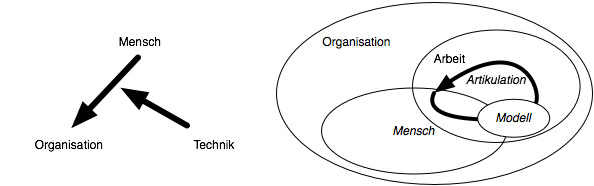
\includegraphics[width=15cm]{img/ExkursMOT/untersuchungsgegenstand.png}
	\caption{Untersuchungsgegenstände}
	\label{fig:img_untersuchungsgegenstand}
\end{figure}

In den folgenden Absätzen werden nun die einzelnen Untersuchungsgegenstände detailliert und in das „MOT“-System eingeordnet. Zusammenfassen kann gesagt werden, dass untersucht wird, welche Auswirkungen der Einsatz von Modellen für arbeitende Menschen bei der Artikulation ihrer individuellen Sicht auf ihre Arbeit hat und wie dieser 

\paragraph{Modell} % (fold)
\label{par:modell}

Modelle (also diagrammatische Repräsentationen) von Arbeit werden in dieser Arbeit eingesetzt, um Individuen (\emph{M}) ihre Arbeit (\emph{O}) -- also jene organisationalen Abläufe in die sie involviert sind, sowie deren Kontext -- abzubilden. Modelle sind hier also individuelle Instrumente, die verwendet werden, um organisationale Phänomene zu beschreiben. In diesem Zusammenhang ist zu untersuchen, welche Eigenschaft die Repräsentationsform der Modelle aufweisen muss, um die Repräsentierbarkeit beliebiger individueller Sichten in Modellen gewährleisten zu können. Dies entspricht im wesentlichen der Beziehung zwischen \emph{M} und \emph{O} in Abbildung \ref{fig:img_untersuchungsgegenstand}.
% paragraph modell (end)

\paragraph{Mensch} % (fold)
\label{par:mensch}

Der Mensch (\emph{M}) als Träger von Arbeit (d.h. als ausführende Instanz) und gleichzeitig als artikulierende (d.h. im Kontext dieser Arbeit: modellierende) Instanz steht im Zentrum der Betrachtungen dieser Arbeit. Untersucht werden muss, wie Menschen Modelle von Arbeit erstellen (können), wie sie diese interpretieren und welche Anforderungen sowohl aus organisationaler (\emph{O}) als auch aus technischer (\emph{T}) Sicht jeweils erfüllt sein müssen, um diese Abläufe zu unterstützen. Dies entspricht im wesentlichen dem Knoten \emph{M} in Abbildung \ref{fig:img_untersuchungsgegenstand}.

% paragraph mensch (end)

\paragraph{Artikulation} % (fold)
\label{par:artikulation}

Als Artikulation wird jener Vorgang bezeichnet, bei dem Menschen (\emph{M}) individuell oder kollektiv ihre Sichten auf ihre Arbeit (\emph{O}) reflektieren und ggf. anpassen bzw. abstimmen -- dieser Prozess ist gleichzeitig integraler Bestandteil von Arbeit selbst. Hier wird einerseits untersucht, wie dieser Artikulationsprozess durch den Einsatz von Modellen (diagrammatischen Repräsentationen) ermöglicht bzw. erleichtert wird und wie die Erstellung der Modelle technisch (T) unterstützt werden kann. Dies entspricht im wesentlichen der Beziehung zwischen \emph{T} und der Kante \emph{M-O} in Abbildung \ref{fig:img_untersuchungsgegenstand}. Zusätzlich ist zu untersuchen, wie sich die Arbeit (\emph{O}) aus Sicht der handelnden Menschen (\emph{M}) durch die Artikulation verändert hat.

% paragraph artikulation (end)